\chapter{Related Work}
\label{chapter:relatedwork}

\section{Social Engineering}

In most companies and private networks, the main focus on security aims towards
secure technology, like firewalls or anti-virus programs and other defense
strategies. However, companies and private persons often are unaware of social
engineering, which sometimes is a lot more dangerous than the IT-security
suggests. Kevin Mitnick, a famous Hacker and one of the most famous social
engineers, states that it is often easier to use social engineering to get
access to a system than searching for security holes \cite{mitnick2003}.

The new hacker's dictionary \cite{raymond1996} defines the term social engineering as
following:
\begin{quote}
\textit{
\glqq{}Term used among crackers and samurai for cracking techniques that rely on
weaknesses in wetware rather than software; the aim is to trick people into
revealing passwords or other information that compromises a target system's
security. [\dots]\grqq{}}
\end{quote}

Beside the definition it is also important to understand, how a social engineer
relates to a hacker in general. \cite{thornburgh2004} proposes, that social
engineers are not hackers themselves, but are \textit{hacker-enablers}.  The
goal of the social engineer is to gain either physical or digital direct access
to an information of the target or an information system.  Afterwards the
social engineer can enable a hacker to access and penetrate the system, delete,
alter and steal information and to disrupt services, as \cite{thornburgh2004}
shows. The social engineer can of course be also the hacker. \cite{jones2004}
states, that unlike hacking, social engineering uses psychology and theories
about the human mindset, like what people expect from each other and their
natural tendency to be helpful.

\subsection{The cycle of an social engineering attack}

Defining the profile of an social engineering attack is quite difficult, as
every attack includes people, who are not discrete like a computer, but their
behaviour changes from time to time, their mood and other things. However,
\cite{mitnick2003} identified four stages of a social engineering attack:
research, developing rapport and trust, exploiting trust and utilizing
information. A single cycle does not have to be limited to a singular cycle, but
can contain several other cycles until the objective is reached, as
\cite{thornburgh2004} states. The process itself can be therefore recursive and
iterative, depending on the attack and used methods.


\begin{figure}
  \begin{center}
    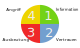
\includegraphics[width=0.75\textwidth]{cycle}
    \caption{A tipical social engineering attack cycle}
  \end{center}
\end{figure}

\subsubsection{Research}

This phase consists of several methodologies to gain as much information about
the target as possible. Depending however if the target is a company or a
private person, different methods might be used. The ultimate goal of this
phase is to gain as much information as possible to develop a relationship,
rapport and trust in the next phase. Of course, there are enormous
possibilities to get information about companies and individuals, the most
known are described by \cite{jones2004,mitnick2003,thornburgh2004}, but of
course are not limited to those.

\begin{description}[\setlabelphantom{Personal Homepage}]

\item[Corporate Website] The Website of a company might be the first place to
  start looking out for information. Lists of employees,
  company directors, or company brochures are often viewable on such websites. 
\item[Personal Homepage] If the target is an individual, the personal homepage
  of the target might offer more information, than the company website. If the
  target is running a blog, information about the workplace can be accessed
  also quite often. This information however can be used to attack the
  employer.
\item[Dumpster Diving] This is a technique was and is also used by certain
  information intelligence agencies [CITATION NEEDED]. It included the search
  for useful information in the dumpster of companies and individuals. While
  this seems a strange technique, a social engineer still can gain much
  information out of this.
\item[Phishing] Fake e-mails or websites are set up and send or accessed by
  individuals. They both have the goal to make the target believe, that they are
  watching a regular e-mail or website and entering sensitive information.
  Phishing can also be described as a whole social engineering attack, however
  it can also be used to just get special information.
\item[Trojan Horses and other Malware] This tools have the same goal like
  phishing, however they are acting by themselves and often do not require any
  user interaction, except might for installing the software. Again, they can
  be used for other things as well, but for example a keylogger or a tool,
  which logs the website the target is accessing or the e-mails can be
  important information too.
\item[Newsgroups and mailing lists] Several employees or individuals are
  subscribed to public accessible newsgroups and mailing lists. Often these are
  technical groups and lists and therefore expose information, like what system
  is getting used and how it is configured.
\item[Job Sites] Companies are often looking for new people to hire and many
  times, they have to include sensitive information, if they are looking for
  people with experience in that field. Like above, information about the
  computer systems can also be obtained here.
\end{description}


\subsubsection{Rapport and trust}

In this phase, the social engineer will make contact via several ways of
communication. The attacker uses techniques like name-dropping, where he will
\textit{drop} several names of verifiable employees or persons to make the target
believe, the attacker is who he pretends. Once the attacker has established
himself as authentic, he will go on with the next phase. \cite{jones2004} shows
the following physical settings, an attack can happen:

\begin{description}[\setlabelphantom{Workplace}]
\item[Telephone] The most common type of social engineering attacks are those
  made by using the telephone. Quite every person is vulnerable to this type,
  especially call desks, but also individuals and employees.
\item[Workplace] This is a quite dangerous type, as an attacker has to gain
  physical access to the targets workplace. However, there are many
  possibilities, a talented attacker can gain legitimate access to a building.
  Once inside, the attacker can look out for passwords, sensitive documents,
  do shoulder-surfing or access computers and network, which are left
  accessible unguarded.
\item[E-Mail] The social engineer can compose an original looking document,
  either from the company, the target works for, another company or a service,
  the target uses, like a social network.
\item[Chat] Like the above, the attacker connects to the victim directly,
  forcing the target to install malicious software or exposing sensitive
  information.
\end{description}


\subsubsection{Exploiting trust}

Once the connection has been established, the attacker can exploit the trust by
\glqq{}weaving a story that plays upon the emotions of the
victim\grqq{} \cite{thornburgh2004}. Social engineers heavily rely on
psychology to exploit their trust. \cite{jones2004} lists the following:

\begin{description}[\setlabelphantom{Workplace}]
\item[Authority] This is can be a highly effective psychological weapon, for
  example when impersonating the boss of the company. \cite{orgill2004} has
  showed in a real case study, that social engineering attacks are even more
  effective, when the supervisor of an employees supports the attack or and
  attacker impersonates a supervisor.
\item[Natural tendency to be helpful] Psychology shows, that it is a natural
  tendency, to be helpful. A social engineer can use this to his advantage.
  Several examples are showed by \cite{mitnick2003}, like desperate calls in
  the night to the help desk, or a person with many boxes in his hand, trying
  to get access to the building.
\item[Liking and similarity] A personal connection might be helpful for the
  attacker. Psychology shows, that it is natural to like people who are like
  themselves. If information about hobbies or interests are available, a social
  engineer might use that information to establish a relationship based on that
  information. Once this connections has been made, the victim may feel more
  responsive to the attacker and therefore might be offer more sensitive
  information.
\item[Reciprocation] Social interaction is often based on the fact, that if
  someone gives something, one might give him something back. In social
  engineering, this is called \textit{reverse social engineering}. Here, a
  social engineer tries to help the victim and in return requests a favour of
  the victim.
\item[Low involvement] If a person has low to no involvement in the company or
  to a victim, it might have little interest in what the social engineer is
  asking. Often, receptionists, the cleaning crew and similar people are the
  favourite victims.
\end{description}

\subsubsection{Utilizing Information}

This phase finally utilizes the gained information to either implement a
technical attack or to use the gained information for a new social engineering
attack \cite{thornburgh2004}. The actual attack and the threat it exposes is
created in this phase. It is interesting, that the attack created here, does
not limit itself to technical attacks, but can also be used to publish
sensitive information or other.

\subsection{Threats and risks through social engineering attacks}

\cite{thornburgh2004} defines a social engineering attack as successful, if the
attacker gets what he wants, even if the information itself is either not
enough to perform a penetration of the target or if the information is
considered of not a great value by the target. Moreover, every bit of
information can help the attack to become successful and increases the
possibility of an successful attack.

\cite{orgill2004} says, that social engineering is an ever-present threat to
the security of computer systems, because it does not attack the computer
itself, but the human being using the computer. It exploits the natural
tendency of humans to trust others, helping them, and gain favour.

In an introduction to social engineering, \cite{manske2000} offers the following:

\begin{quote}\textit{
Successful social engineering attacks give the attacker the means to bypass
millions of dollars invested in technical and nontechnical protection
mechanisms and consulting, completely nullifying security investment,
Firewalls, secure routers, PKI, e-mail\dots and security guards are all down
the drain. 
} \end{quote}

The risk of of a social engineering attack depends mostly on the value of the
gained information, as \cite{thornburgh2004} states. If the gained information
cannot help to develop another attack, the impact of this special attack is
minimal to non-existent. On the other side, valuable information can lead to a
very dangerous attack, especially if the attacker remained hidden and the
attack has not been detected throughout his attack. If the attacker was not
able to remain hidden, a system penetration is still possible, however
subsequent attacks can be prevented possibly. Overall, a social engineering
attack can be as dangerous as the information gained. However, non valuable
information still can help the social engineer to acquire more valuable
information.

It was shown, that a typical social engineering attack is cyclical and
therefore can be repeated inside a company or using several individuals. The
target can be penetrated over and over again, until the ultimate goal is
reached. Also different goals are possible here. \cite{thornburgh2004} and
\cite{mitnick2003} both mention, that social engineers take care to keep the
target for further attacks or not to \textit{burn} it, as \cite{thornburgh2004}
calls it. They try to remain anonymous and to do everything to prevent their
detection.

Amongst several others, \cite{mitnick2003}, \cite{orgill2004} and
\cite{winkler1995} showed how easy it is, to get access to a company. They used
several methods, like telephone, surveys and other. All were extremely
successful and while not being expensive, all of those case studies managed to
get sensitive information in a very short amount of time, despite strong
security measures. All of these did not use very company specific data, and the
case studies can easily extrapolated to other attacks at other companies.

\subsection{Countermeasures against social engineering attacks}

\cite{winkler1995} showed, that many of the weaknesses exploited by the
attackers were common to most companies. Though they mention, that even the
best technical mechanisms had not prevented the attacks. The attacker exploited
poor security awareness, and even if the attackers would not have been able to
get passwords, they still would have been able to acquire sensitive personal
and company information.

Moreover, security operators have to consider the non-technical side of
computer security, and not assume, that for example cryptography is enough to
prevent attacks. Then, computer professionals believe all to often, that
computer security fundamentals are known to everyone. \cite{lively2003} hits
the point with the following: \textit{\glqq{}Users cannot defend against what
they do not know\grqq{}}. Most of the related work sees user awareness and user
rewards as essential part against social engineering, however they agree, that
there is no way to protect themselves against social engineering attacks.

\cite{mitnick2003} tries to give some points, how a social engineering attack
can be recognized, however all of these points still can happen in a totally
ordinary phone call or dialogue. Though, they give a good base to recognize
attacks.

\begin{itemize}
  \item Refuses to give a callback number
  \item Out of ordinary request
  \item Claim of authority
  \item Stresses urgency
  \item Threatens negative consequences
  \item Show discomfort when questioned
  \item Name dropping
\end{itemize}

\cite{winkler1995} tries to create a more concrete policy with the following
points:

\begin{description}
  \item[Do not rely upon common internal identifiers] Some companies use basic
  authentication methods to authenticate as real employees. Unfortunately the
  employee number or similar identifiers are commonly used by companies.
  Therefore it is quite easy to get a list or just some single identifiers and
  use them for authentication. The authors suggest having a different
  identifier for computer related activities and not to rely upon such simple
  identifiers.
  \item[Implement a call back procedure] Often, social engineering attacks can
  be prevented, if employees would have verified the caller identity by calling
  them back at their proper number, as listed in the company directory. This of
  course also includes e-mail or instant messaging. Though it creates an
  inconvenience, but when compared to the potential losses, this is of course
  justified, as the team shows. Caller ID services or reverse DNS services can
  be helpful too.
  \item[Implement a security awareness program] Companies often spend an
  enormous amount of money on hard- and software security devices. Still, security
  awareness programs are seldom implemented. As stated before, computer
  professionals cannot assume, that security practises, even the simplest, are
  known to every user. The paper also mentions, that a good security awareness
  program can be implemented for minimal cost and can save a lot of money,
  compared to the losses.
  \item[Identify direct computer support analysts] In a company, every employee
  should be familiar with a single well known computer analyst. This analyst on
  the other side, should not have more than 60 users. He should be the only
  person, who should contact and should be contacted by the users. The users
  should also contact their computer analyst immediately, if another person
  from the computer support should contact them.
  \item[Create a security alert system] During the attacks, the authors did,
  they recognized, that there was no way to warn other employees, if a single
  employee of the company would have detected them. So, the attack could
  continue, until their goal was reached, even if they were detected by some
  employees. They also mention, that a detection would only have improved the
  attack, as the attackers would have learned what works and what does
  not.InDuring the attacks, the authors did, they recognized, that there was
  no way to warn other employees, if a single employee of the company would
  have detected them. So, the attack could continue, until their goal was
  reached, even if they were detected by some employees. They also mention,
  that a detection would only have improved the attack, as the attackers would
  have learned what works and what does not.
  \item[Test security policies] While already many people test their physical
  and electronical security devices, the human vulnerabilities are often not
  touched. But to enable the above mentioned policies, they have to be tested
  by social engineering attacks for their effectiveness. And then still, those
  policies cannot assure 100\% protection against social engineering attacks.
\end{description}

\section{Bridging the gap}
